\section{Normal Distribution Dataset}

\subsection{Part A: Developing Hypotheses}
Identify and collect a real-world dataset that you hypothesize follows a Normal distribution. Please be clear about the reasoning behind your hypothesis and be specific about the source of the dataset.\\
-----\\
We have collected the Iris dataset for this example. Specifically, we will use the sepal widths of the Setosa species in the dataset. We hypothesize this data to follow a Normal distribution because the sepal widths of Setosas ought to be influenced by many underlying environmental factors. These factors could be anything from the composition of the soil, the level of shade, the composition of the surrounding ecosystem, the agricultural practices of surrounding human civilizations, etc. More generally, notions of performance in a homogenous population often approximate a Gaussian, as most observations will tend to distribute about the mean, symmetrically deviating from the general behavior on each side of the spectrum, becoming less frequent at extreme conditions. The Iris dataset was originally produced by Ronald Fisher in 1936 and was sourced from \hyperlink{https://www.kaggle.com/datasets/uciml/iris}{this page} on Kaggle.\\

As our hypothesize relates to the Gaussian distribution PDF:

$$
f(x) = \frac{1}{\sigma \sqrt{2\pi}} e^{ -\frac{1}{2} \left( \frac{x - \mu}{\sigma} \right)^2 } 
$$

The model defines a mean parameter $ \mu $ that the distribution mass is centered around, reflecting the idea that the sepal widths are going to average to some value over the observations. The exponential term $ e^{ -\frac{1}{2} \left( \frac{x - \mu}{\sigma} \right)^2 } $ defines the decay behavior for the Gaussian, dictated by the standard deviation parameter $ \sigma $. The difference between the observation $ x $ and $ \mu $ is squared so that deviations from the mean decay exponentially and symmetrically about the center, which are then scaled relative to the variance $ \sigma^2 $, i.e. the general proclivity of a population to deviate from its mean.\\ 

In other words, if the distribution of mass for some population tends to deviate from the mean naturally (higher $ \sigma^2 $ ), then the decay for observations far from the mean is much slower. This captures the natural variance of the observations in our data, and the bell shape reflects the fact that many Setosas ought to have generally similar sepal widths, and extreme cases ought to be less and less common the more extreme the observations get.\\
\newpage

\subsection{Part B: Fitting Distributions}
For this exercise, we will call each of the four different theoretical distributions (normal, uniform, power law, exponential) a ``model". Fit the dataset (i.e., estimate the model parameters) against each model (not just the one you hypothesized) using maximum likelihood estimation (or using any technique you think is appropriate; make sure to comment on the validity of your approach). This should result in a total of \textbf{4 parameter sets}. Report the estimated parameters in the following tabular format:

\begin{center}
\begin{tabular}{|c|c|c|c|c|c|}
\hline
& & \multicolumn{4}{c|}{{\bf{\em{Model}}}}\\
\hline
{{\bf{\em{Dataset}}}} & {\bf{\em{\# Observations}}} &\textbf{Normal}& \textbf{Uniform} & \textbf{Power law} & \textbf{Exponential} \\
\hline
\textbf{Dataset 1} & $n_1$ &  $\mu_1, \sigma_1$ & $a_1, b_1$ & $\alpha_1, x_{\min_1}$ & $\lambda_1$ \\
\hline
\end{tabular}
\end{center}

Be sure to show the code you used to arrive at your final estimates clearly.\\
-----\\
Below is the code that produced the parameter estimates and the tabulated estimates for this dataset (for the full tabulation described in the original assignment TeX, see Appendix):

\begin{verbatim}
def dists_fit(input_csv: str) -> tuple:
    """
    Fits the obs dataset to each model using MLE.

    :param input_csv: Path to input data to fit paramater(s) to
    :type input_csv: str
    """
    obs = pd.read_csv(input_csv).iloc[:, 0].to_numpy()

    mu = np.mean(obs)
    std = np.sqrt(np.sum((obs - mu) ** 2) / len(obs))

    a, b = obs.min(), obs.max()

    alpha = 1 + len(obs) / np.sum(np.log(obs / a))

    lamb = 1 / np.mean(obs)

    return (mu, std, a, b, alpha, lamb)
\end{verbatim}

\begin{center}
\textbf{Figure 1:} Parameter estimation function for the four models.
\end{center}

\begin{center}
\begin{tabular}{|c|c|c|c|c|c|}
\hline
& & \multicolumn{4}{c|}{{\bf{\em{Model}}}}\\
\hline
{{\bf{\em{Dataset}}}} & {\bf{\em{\# Observations}}} &\textbf{Normal}& \textbf{Uniform} & \textbf{Power law} & \textbf{Exponential} \\
\hline
\textbf{Iris Sepal Widths (Setosa)} & 50 &  3.4, 0.4 & 2.3, 4.4 & 3.6, 2.3 & 0.3 \\
\hline
\end{tabular}
\end{center}

\begin{center}
\textbf{Figure 2:} Parameter estimates for each model on Iris Sepal Widths (Setosa).
\end{center}
\newpage


\subsection{Part C: Comparing Real and Synthetic Data}

For each fitted distribution (there will be 4 of them for this dataset, each corresponding to a different model), generate a synthetic sample of data points equal to the sample size of the real dataset using the respective model parameters you inferred from the real dataset.\\

Compare the real vs. synthetic data distributions using methods you think are the most appropriate, including visualizations. So, for this dataset, we compare the original dataset to four synthetic datasets, all with equal number of observations, but each synthetic dataset is generated using a different model.\\

For this dataset, identify the synthetic dataset (which corresponds to a model) that is most similar to the original data in terms of its distribution.\\

Now revisit your initial hypothesis. For this dataset: Did the dataset behave as expected, or was another model (assumed distribution) a better fit to the dataset? Reflect on why the observed results may differ from your expectations.\\ 
-----\\
Below is the code that produced the synthetic datasets for each fitted distribution:

\begin{verbatim}
def dists_generate(input_csv: str, params: tuple, dist_type: str):
    """
    Generates N synthetic examples

    :param input_csv: Path to input dataset
    :type input_csv: str
    :param params: tuple of parameters returned by dists_fit (mu, std, a, b, alpha, lamb)
    :type params: tuple
    :param dist_type: name of the folder correponsding to a type of distribution
    :type dist_type: str
    """
    obs_df = pd.read_csv(input_csv)
    obs_name = obs_df.columns[0]
    obs = obs_df.iloc[:, 0].to_numpy()
    n = len(obs)

    mu, std, a, b, alpha, lamb = params

    gaussian_samples = int(np.random.normal(loc=mu, scale=std, size=n))
    uniform_samples = int(np.random.uniform(low=a, high=b, size=n))
    powerlaw_samples = int((a * (1 - np.random.uniform(0, 1, n)) ** (-1 / (alpha - 1))))
    exponential_samples = int(np.random.exponential(scale=1/lamb, size=n))

    gaussian_df = pd.DataFrame({f'{obs_name}_gaussian': gaussian_samples})
    uniform_df = pd.DataFrame({f'{obs_name}_uniform': uniform_samples})
    powerlaw_df = pd.DataFrame({f'{obs_name}_powerlaw': powerlaw_samples})
    exponential_df = pd.DataFrame({f'{obs_name}_exponential': exponential_samples})
    
    gaussian_df.to_csv(f'../datasets/{dist_type}/synth/{obs_name}_gaussian.csv', index=False)
    uniform_df.to_csv(f'../datasets/{dist_type}/synth/{obs_name}_uniform.csv', index=False) 
    powerlaw_df.to_csv(f'../datasets/{dist_type}/synth/{obs_name}_powerlaw.csv', index=False)
    exponential_df.to_csv(f'../datasets/{dist_type}/synth/{obs_name}_exponential.csv', index=False)
\end{verbatim}

\begin{center}
\textbf{Figure 3:} Sampling function for fitted distributions.
\end{center}

We believe an appropriate test for these synthetic distributions would be the K-S statistic because we can equip ourselves with a notion of disagreement between the distributions in terms of their maximum difference between the cumulative probability structure of the actual dataset. The K-S test implemented in SciPy also provides the p-value for our comparisons, so before evening looking at the distributions we can gauge the disagreement between synthetic and real and the extent to which that disagreement is structurally significant or if it's just a product of random noise.\\

We can see in the table below that immediately the Power Law and Exponential models stand out tremendously with K-S statistics above and around 0.5, both of which are disagreements that are very structural in nature. On the other hand, the Uniform and Normal models show much less disagreement in their CDFs relative to the real sample, however the difference in p-value is very telling of which is actually representative of the data. The 0.04 p-value for the Uniform distribution tells us immediately that there is almost no chance, a 3.9\% probability, that such as disagreement could come from two samples in the same distribution, whereas the p-value for the Normal suggests there you could see this K-S statistic with about a 96.7\% chance if the two samples were pulled from the same distribution.\\

Without even observing the other two visualizations we prepared, we can make quite strong claims about which models do well to represent that Sepal Widths dataset and which do not, though it is always helpful to pair these statistics with a visualization that makes the comparison much more readily obvious. In Fig 5, we observe that the Power Law and Exponential models at least begin to converge, climbing a little bit of the probability mass of the real data, but the Uniform and Normal models clearly outmatch them with central tendencies much closer to the real sample.\\

\begin{center}
\begin{tabular}{|c|c|c|c|}
\hline
\textbf{Distribution} & \textbf{K-S Statistic} & \textbf{p-value} & \textbf{Significant} \\
\hline
Normal & 0.10 & 0.967 & No \\
\hline
Uniform & 0.28 & 0.039 & Yes \\
\hline
Power Law & 0.48 & 1.39 $\times 10^{-5}$ & Yes \\
\hline
Exponential & 0.64 & 6.08 $\times 10^{-10}$ & Yes \\
\hline
\end{tabular}
\end{center}

\begin{center}
\textbf{Figure 4:} Kolmogorov-Smirnov test results between Sepal Widths dataset and synthetic samples.
\end{center}

The histogram also makes it readily obvious the disparity between the Uniform and Normal. While the Uniform performs in a different class than the previous two models, it remains apparent from the mass distribution that the Uniform distribution is more right-skewed and not as centered about its mean as the real sample.\\

\begin{center}
  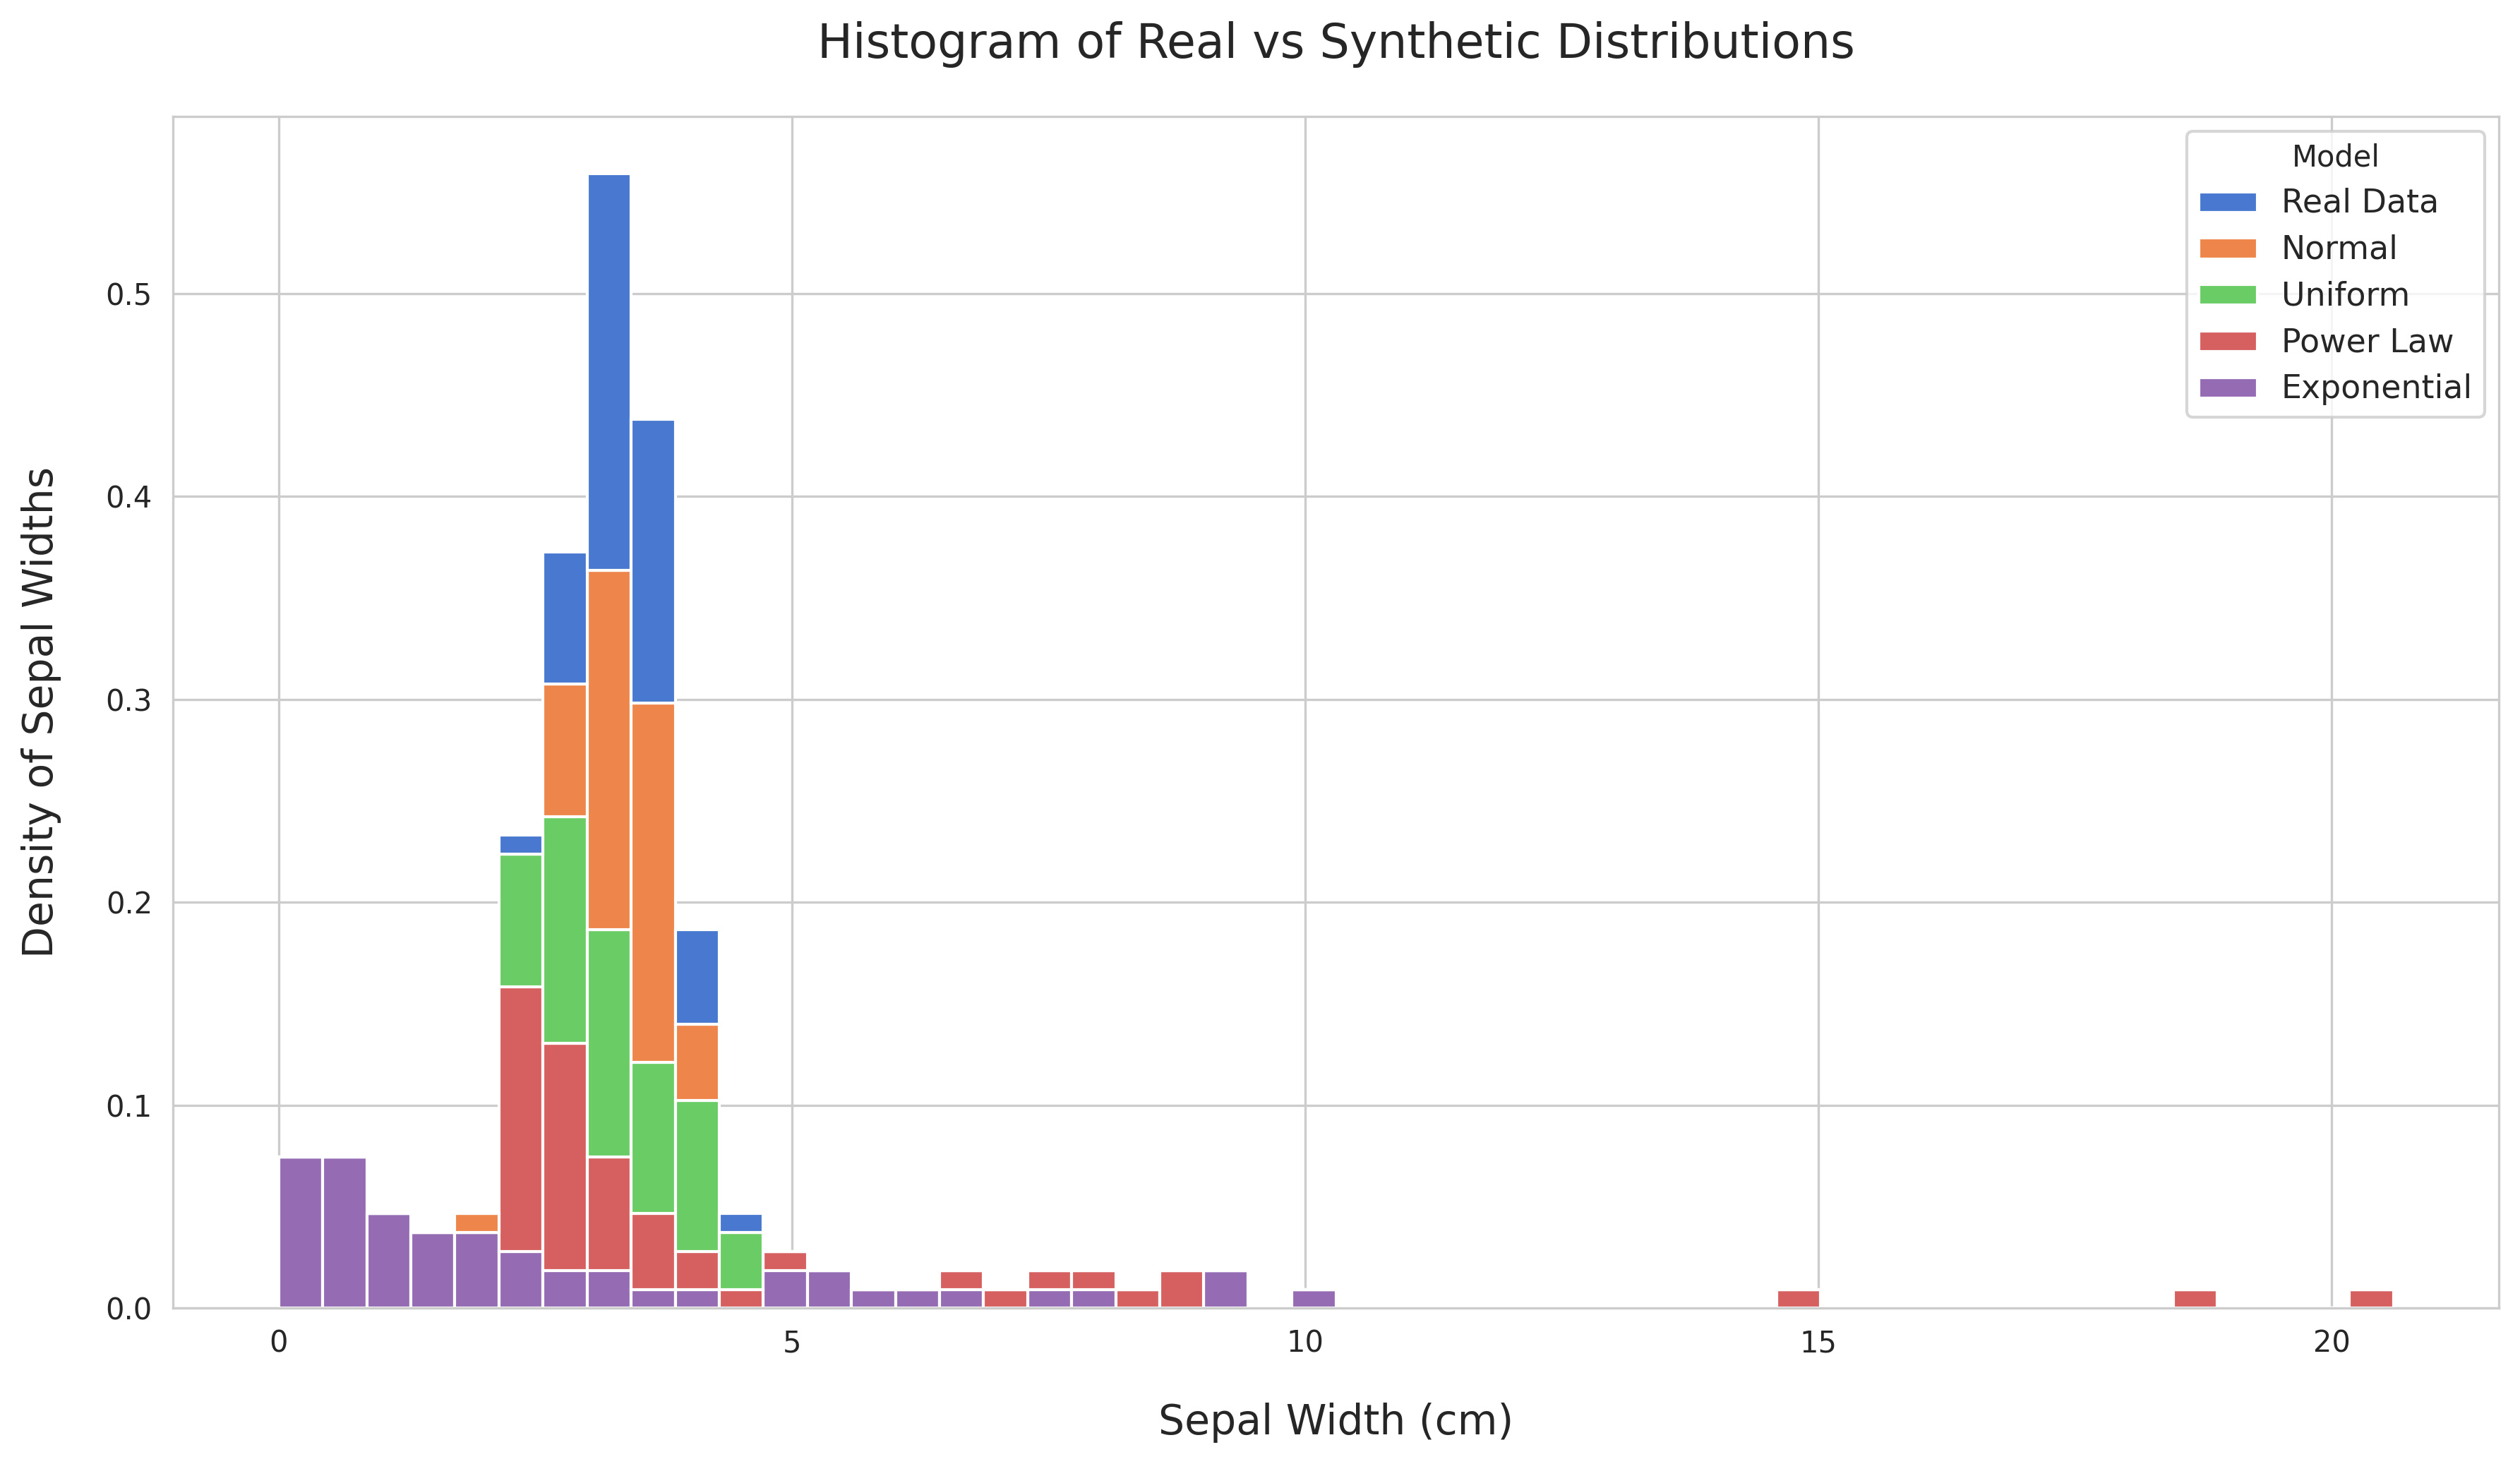
\includegraphics[width=0.95\textwidth]{figures/normal/histogram.png}
  
  \textbf{Figure 5:} Histogram of Real vs Synthetic Distributions on Sepal Widths dataset.
\end{center}

To better confirm the comparison between the Uniform and Normal Distribution, we also curated a Q-QPlot of the data over 25 quantiles to gauge the agreement between the real and synthetic samples across the entire distribution. What we are left with is a general agreement of each model with the real sample's quantiles for average-case behavior, but the Uniform shows an obvious "snaking" pattern about the agreement line that worsens toward the extremes of the distributions.\\ 

\begin{center}
  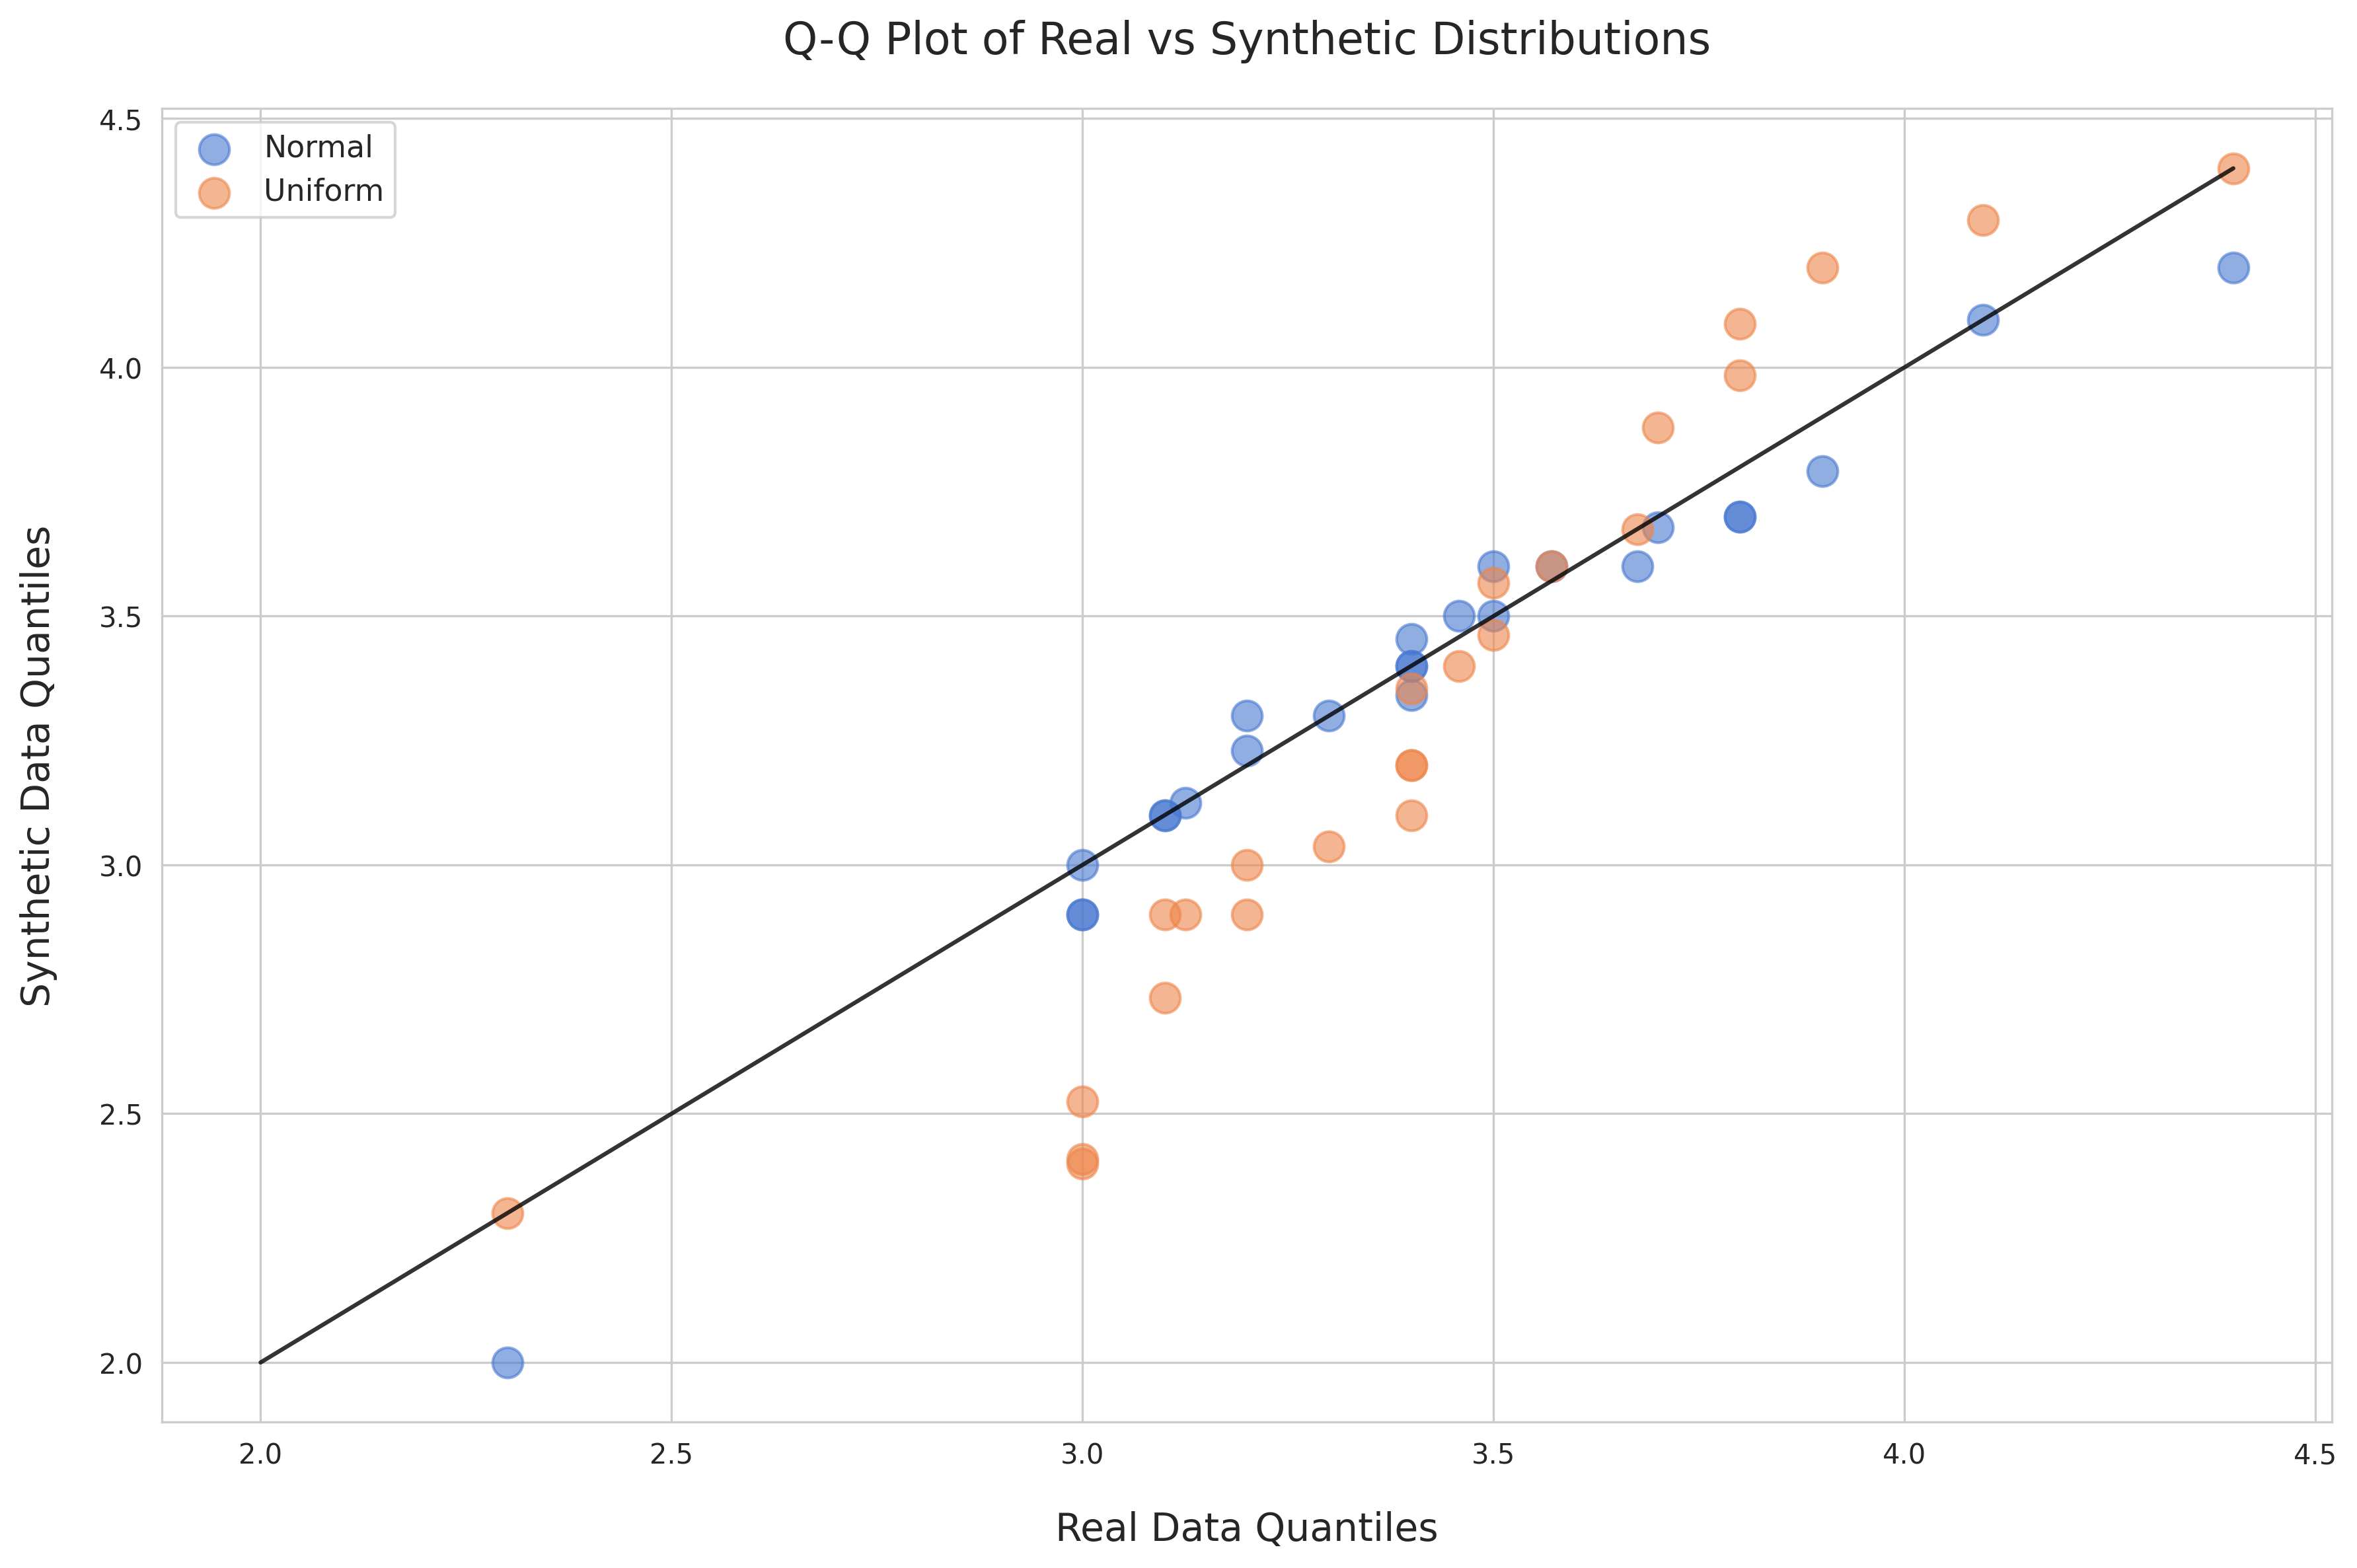
\includegraphics[width=0.95\textwidth]{figures/normal/qqplot.png}
  
  \textbf{Figure 6:} Q-Q Plot comparing Real vs Synthetic quantiles on Sepal Widths dataset.
\end{center}

Given these comparisons, we can make a strong claim that the sepal\_widths\_gaussian synthetic dataset is most similar to the real data in terms of its distribution. This aligns with our original claim that the Sepal Widths dataset contains notions of central tendency and a spread about its mean that decays toward extreme values.
\newpage
